%---------------------------------------------------------------------------------------------------
% Hauptteil
%---------------------------------------------------------------------------------------------------
\section{Hauptteil} 

\subsection{Der Token Ring Algorithmus}
Der Token Ring Algorithmus ist ein Wahlalgorithmus der von Chang und Roberts 1979 entworfen wurde. Er kann verteilt auf mehreren Clienten verwendet werden die in einer Ring-Topologie miteinander verbunden sind. Das Ziel des Algorithmus ist, bei Ausfall des Master-Clienten im Netz einen neuen zu wählen.

\subsubsection*{Voraussetzungen}
Damit der Algorithmus auf eine Ring-Topologie angewandt werden kann, müssen folgende Voraussetzungen im Netz gegeben sein:
\begin{itemize}
	\item Jeder Client kennt seinen Nachfolger
	\item Jeder Client ist mit seinem Nachfolger verbunden, sodass er mit ihm kommunizieren kann
	\item Jeder Client hat eine eindeutige ID
	\item Jeder Client kennt die gesamte Ring-Topologie
\end{itemize}

\subsubsection*{Ablauf}\label{sec:algorithm_process}
Der Algorithmus startet wenn der Master-Client ausfällt. Der Vorgänger des ausgefallenen Master-Clients baut eine Verbindung zum Nachfolger des ausgefallenen Master-Clients auf, sodass die Ring-Topologie wieder vollständig ist.

Der Client, der den Ausfall bemerkt, startet die Wahl in dem er seinem Nachfolger eine Nachricht mit seiner ID und der Info dass es sich um eine Wahl handelt schickt. Dieser nimmt die Nachricht und überprüft ob seine eigene ID darin vor kommt. Falls nicht, hängt er seine eigene ID hinten an und schickt die vervollständigte Nachricht an seinen Nachfolger.

Wenn ein Client feststellt, dass seine eigene ID bereits in der Nachricht vorhanden ist, nimmt er die höchste ID aus der Liste der gesammelten IDs in der Nachricht. Anschließend sendet er eine "Gewählt"-Nachricht mit der höchsten ID an seinen Nachfolger. Der Empfänger der "Gewählt"-Nachricht merkt sich, dass der gewählte Client nun der neue Master ist und sendet seinem Nachfolger die gleiche "Gewählt"-Nachricht. Jeder wird somit benachrichtigt was die höchste ID ist. Kommt die "Gewählt" Nachricht wieder am Initiator der "Gewählt"-Nachricht an, wird die Wahl erfolgreich beendet und der Algorithmus ist terminiert.

\subsubsection*{Eigenschaften}
Die Laufzeit dieses Algorithmus befindet sich in einem Bereich von $0=2N$ wobei N die Anzahl der teilnehmenden Clienten ist. Diese Einschätzung ergibt sich daraus, dass es zwei Nachrichten gibt die jeweils einmal jeden Clienten erreichen müssen. Dabei durchläuft die erste Nachricht, die Wahl N Clienten und die Nachricht, dass ein neuer Master gewählt wurde durchläuft ebenfalls noch einmal N Clienten.
 
Die Eigenschaften des Algorithmus lassen sich wie folgt beschreiben
 \begin{itemize}
	\item Laufzeit von 2N
	\item 2 Arten von Nachrichten "Wahl"-Nachricht mit ID Liste und "Gewählt"-Nachricht mit der neuen Master ID
	\item Der Algorithmus findet in einer endlichen Anzahl von Clienten immer den neuen Master (höchste ID)
	\item Alle Teilnehmenden Clienten setzten irgendwann ihren Master auf den gewählten Master 
	\item Der Algorithmus terminiert sicher
\end{itemize}
%%Welche Grundlegenden Eigenschaften hat der Algorithmus
%%was tut er und warum, wofür?

\subsection{Spezifikation}
Damit ein Modell erstellt werden kann, das den Algorithmus abbildet, müssen zunächst die charakteristischen Eigenschaften des Algorithmus bestimmt werden.

Der Algorithmus (s. Abschnitt \ref{sec:algorithm_process}) lässt sich in folgende drei Phasen einteilen:
\begin{description}
\item[Phase 1:] Ein Client bemerkt den Ausfall des bisherigen Masters
\item[Phase 2:] Sammeln aller beteiligten Client-IDs
\item[Phase 3:] Bekanntgeben des neuen Masters
\end{description}

Der jeweilige Ablauf der Phasen lässt sich mit folgenden Punkten spezifizieren:

\begin{table}[H]
\begin{tabular}{|c|p{7,6cm}|c|}
\hline Phase & Eigenschaft & Nr.\\ 
\hline Phase 1: Master-Ausfall bemerkt & Sendet Nachricht zum Wählen und hängt seine eigene ID daran & 1\\ 
\hline \multirow{3}*{Phase 2: Wahl} & Client, der Wahl-Nachricht erhält, hängt seine eigene ID an die Nachricht & 2\\ 
\cline{2-3} & Client sendet die erweiterte Nachricht an seinen Nachfolger & 3\\ 
\cline{2-3} & Sobald ein Client eine Wahl-Nachricht erhält, in der seine eigene ID bereits enthalten ist, geht der Algorithmus in Phase 3 über & 4\\ 
\hline \multirow{3}{*}{Phase 3: Neuen Master mitteilen} & Der Client, der feststellt, dass Phase 2 vorbei ist, sendet eine Nachricht mit dem neuen Master an seinen Nachfolger & 5\\
\cline{2-3} & Ein Client, der die Nachricht über einen Master erhält, merkt sich den neuen Master & 6\\ 
\cline{2-3} & Ein Client, der die Nachricht über einen Master erhält, teilt seinem Nachfolger diese Nachricht mit & 7\\
\cline{2-3} & Sobald der Client, der Phase 3 eingeleitet hat, die Nachricht über den neuen Master erhalten hat, terminiert der Algorithmus & 8\\
\hline 
\end{tabular}
\caption{Spezifikation der Phasen des Algorithmus}
\label{table: algorithm_specification} 
\end{table}

\subsection{Modellierung}

Für die Modellierung wurde der Algorithmus mithilfe der Spezifikation auf seine essentiellen Bestandteile untersucht und an die Möglichkeiten von Petri Netzen angepasst. Es musste ebenfalls verarbeitet werden, dass die Möglichkeiten des zu verwendenden Programms \textit{Snoopy} hinsichtlich des Umfangs und der Mächtigkeit der Petri Netze eingeschränkt ist. So konnten zum Beispiel die ID Listen in den Nachrichten nicht umgesetzt werden. 


Einige Eigenschaften des Algorithmus bereiten Probleme wenn sie in einem normalen Petri Netz abgebildet werden sollen. Dazu gehört:
 \begin{enumerate}
 	\item Clienten haben eine eigene ID
	\item Nachrichten übermitteln unterschiedliche Datenstrukturen (Nachrichten Art, ID Listen)
	\item Bei unterschiedlichen Nachrichten reagiert der Client anders
 \end{enumerate}
		 	
Einige dieser Probleme können dadurch gelöst werden indem ein farbiges Petri Netz genutzt wird (CPN). Dieses ermöglicht mithilfe von Farben und Konstanten jedem Clienten eine eigene ID zu geben. Durch Guards an den Transitionen und Variablen kann ein unterschiedliches Verhalten erzeugt werden. Ein Problem das sich damit allerdings nicht lösen lies war die Datenstrukturen, ein Token kann nur einen einzigen Wert haben.

Um dieses Problem zu beheben wurde der Algorithmus ein wenig verändert. Für die Modellierung werden keine ID Listen weiter gereicht sondern nur noch eine einzige ID und zwar die lokal größte. Das bedeutet, der Initiator schickt seine ID zu seinem Nachbarn. Dieser vergleicht die ID mit der eigenen und schickt die Größere weiter. Dies stellt keine Grundlegende Änderung in der Funktionsweise des Algorithmus dar sondern verschiebt bloß den Schritt des Vergleichs. Nun überprüft nicht mehr nur der Initiator welches die höchste ID ist, sondern jeder Client überprüft die eigene ID mit der empfangenen. Wie der Algorithmus nun im Detail abläuft wird im Folgenden beschrieben.

Um den Algorithmus abzubilden wurde ein farbiges Petri Netz gewählt um den Token eine Gewichtung geben zu können die die ID der jeweiligen Clienten widerspiegelt. Des Weiteren war es notwendig an den Transitionen entscheiden zu können wann diese Schalten. Auch dies bietet das farbige Petri Netz (CPN) durch Guards.

%%Wie haben wir ihn modelliert
%%-Gefärbtes netz
%%- Ids
%%- Guards
%%Erklären an wo die spezifizierten Punkte im Netz zu finden sind.


\subsubsection{Das Netz}
In der untenstehenden Abbildung ist das gesamte Netz zu sehen, dass das Ergebnis der Modellierung war. Um eine gewisse Übersichtlichkeit zu wahren wurden nur drei Clienten modelliert. Dies reicht um die Funktionalität des Algorithmus zu modellieren hält aber den Komplexitätslevel und vor allem die Unübersichtlichkeit in Grenzen. 


\begin{figure}[H]
\centering
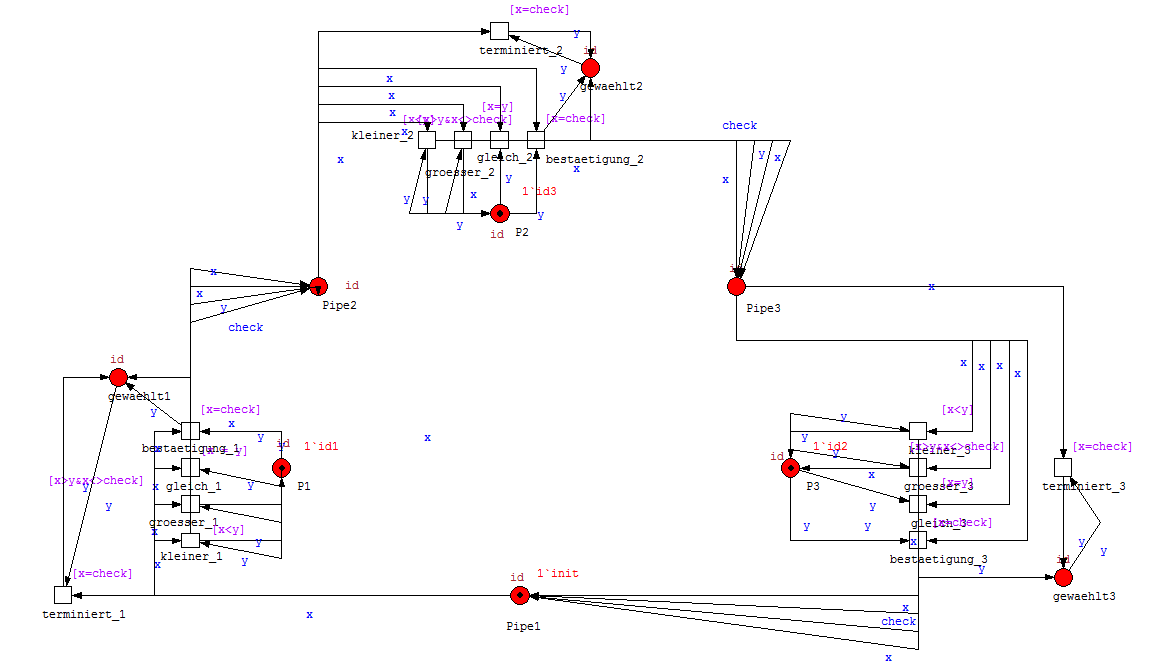
\includegraphics[width=1\linewidth]{kapitel/hauptteil/img/cpn}
\caption{Der Token Ring Algorithmus als farbiges Petri Netz}
\label{fig:cpn}
\end{figure}

Das Netz besteht im Grunde aus einem Konstrukt das den Clienten beschreibt und sich N mal wiederholt, in unserem Fall ist N=3, es gibt also drei Clienten. Die Nachrichtenleitung wurde durch drei Stellen umgesetzt und zwar \textit{Pipe1 - Pipe3} die die Clienten miteinander verbinden. Zwischen diesen Stellen befindet sich jeweils ein aus fünf Transitionen und zwei Stellen bestehendes Konstrukt das jeweils einen Clienten darstellt. Die untenstehende Abbildung zeigt einen Clienten zur Veranschaulichung. 

Ein Client \textit{P{n}} bekommt Nachrichten immer von der Nachrichtenleitung \textit{Pn} und sendet Nachrichten auf die Leitung \textit{Pn+1}. Die ankommende Nachricht am Client hat die Möglichkeit fünf Transitionen zu schalten. Die Guards an den Transitionen sind allerdings so gewählt das niemals alle geschaltet werden können sondern höchstens eine. Den Algorithmus bilden davon vier der Transitionen ab, die fünfte \textit{terminiert\_n} ist dafür da, dass die Token aufhören zu wandern wenn die Wahl getroffen ist und geben die Leitung damit frei. Dies ist eine reine Formsache. Die anderen vier Transitionen vergleichen den Token der von \textit{Pipen} kommt mit dem Token der auf \textit{Pn} liegt. Jede Transition kümmert sich um einen Vergleich \textit{kleiner\_n} überprüft ob der neue Token kleiner ist als der gespeicherte, \textit{groesser\_n} ob der kommende Token größer ist aber nicht so groß wie der 'Gewählt'-Token, \textit{gleich\_n} überprüft ob es der Token ist der bereits gespeichert wurde und \textit{bestaetigung\_n} ermittelt ob es die 'Gewählt'-Nachricht ist. Je nachdem welche Transition schaltet werden unterschiedliche Aktionen ausgeführt. Ist der ankommende Token kleiner (es schaltet \textit{kleiner\_n}) wird er ignoriert und der eigene Token als größerer weitergeleitet, also auf \textit{Pipe\_N+1} gelegt und wieder gespeichert also auf \textit{Pn} geschoben. Ist der kommende Token größer (es schaltet \textit{groesser\_n}) wird der kommende Token auf \textit{Pipe\_N+1} weitergeleitet und in \textit{Pn} gespeichert. Wenn die Transition \textit{gleich\_n} schaltet sind beide Token gleich. Dadurch wird die Phase gewechselt. Also aus der in \ref{table: algorithm_specification} definierten Phase 2 der Wahl in die Phase 3 - Bekanntgeben des neuen Masters, gewechselt. Es wird der 'Gewählt'-Token initialisiert und auf \textit{Pipe\_N+1} gelegt. Der bis eben gespeicherte Token wandert auf die Stelle \textit{gewaehltN}. Die vierte Transition regelt den Fall, dass ein 'Gewählt'-Token kommt. Wenn dies geschieht schaltet die Transition nur in dem Fall, dass der Client die Nachricht nicht selbst initialisiert hat. Nur dann kann die \textit{bestaetigung\_n} Transition schalten. Hat der Client selbst die 'Gewählt'-Nachricht initialisiert liegt auf \textit{Pn} kein Token mehr. In diesem Fall schaltet die \textit{terminiert\_N} Transition und zieht den 'Gewählt'-Token von der Pipe. Diese Transition kann nur dann schalten weil dann bereits der gespeicherte Token auf der \textit{gewaehltN} Stelle liegt.
An dieser Stelle terminiert der Algorithmus und alle Clienten haben die höchste ID auf der \textit{gewaehltN} Stelle liegen.

\begin{figure}[H]
\centering
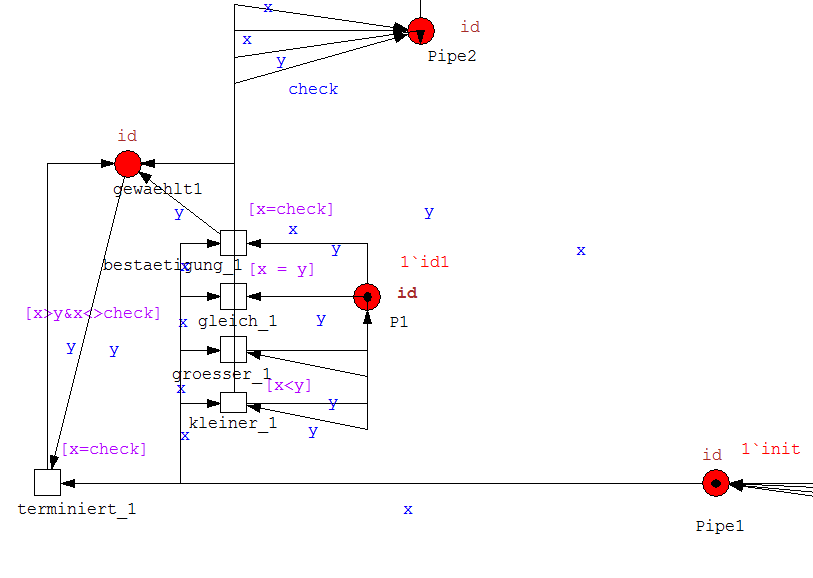
\includegraphics[width=1\linewidth]{kapitel/hauptteil/img/cpn_detail}
\caption{Detailausschnitt eines Clienten}
\label{fig:cpn_detail}
\end{figure}

\subsection{Ablauf}

\textbf{Phase 1 - Master-Ausfall bemerkt}\\
Das Netz ist so konfiguriert das alle Clienten mit ihrer eigenen einzigartigen ID als Token auf ihrem internen Speicher \textit{Pn} starten. Auf der Initiator Stelle \textit{Pipe\_1} liegt ein Token mit einer sehr geringen Wertung. Diese Stelle ist in der Regel eine normale Leitung, durch den Start mit einem Token der Wertigkeit 1 (alle Ids sind größer als 1) initiiert es am Anfang die Wahl in dem der Token zum ersten Clienten wandert der ihn mit seinem eigenen vergleicht.	

\textbf{Phase 2 - Wahl}\\
Nach der Initialisierung läuft ein Token mit der aktuell höchsten ID herum. Dabei überprüft jeder Client bei dem der Token ankommt ob die eigene , bzw gespeicherte ID größer ist. Je nachdem wird entweder die eigene ID weitergeschickt oder die neue und dann auch gespeichert. Stellt ein Client fest das die verglichenen Token gleich sind ist der Token einmal herum gelaufen und die größte ID steht fest. Also schreibt der Client die ID weg und löst die 'Gewählt'-Nachricht aus und startet dadurch Phase 3.

\textbf{Phase 3 - Neuen Master mitteilen}\\
Die dritte Phase ist dafür da, allen Clienten mitzuteilen dass die ID die sie gerade gespeichert haben die endgültige ist. Dies passiert in dem die 'Gewählt'-Nachricht herum geschickt wird. Jeder Client der diese Nachricht erhält schreibt die ID von \textit{Pn} auf die \textit{gewaehltN} Stelle und schickt die 'Gewählt'-Nachricht weiter. Kommt diese Nachricht wieder bei dem Clienten an der sie losgesendet hat schaltet die \textit{terminiert\_n} Transition und nimmt die Nachricht aus der Pipe. Das Netz kann nun nicht mehr schalten und hat an allen Clienten die höchste ID gewähl.

\subsection{Abbildung der Spezifikation in der Modellierung} \label{Spezi-Modell}

Die folgende Abbildung verdeutlicht wie die Spezifikation durch die Modellierung abgedeckt wurde

\begin{table}[H]
\centering
\begin{tabular}{|p{7,6cm}|p{7,6cm}|c|}
\hline Phase und Spezifikiationseigenschaft & Modell Eigenschaft & Nr.\\ 
\hline Phase 1: Sendet Nachricht zum Wählen und hängt seine eigene ID daran & Auf \textit{Pipe1} liegt der Initiator-Token und startet den ersten Vergleich bei Client 1   & 1\\ 
\hline Phase 2: Client, der Wahl-Nachricht erhält, hängt seine eigene ID an die Nachricht & Jeder Client vergleicht und sendet nur die höchste ID & 2\\
\hline Phase 2:Client sendet die erweiterte Nachricht an seinen Nachfolger & Die höhere ID wird auf die \textit{PipeN+1} gelegt die den Token an den nächsten Clienten liefert & 3\\
\hline Phase 2:Sobald ein Client eine Wahl-Nachricht erhält, in der seine eigene ID bereits enthalten ist, geht der Algorithmus in Phase 3 über & Erhält ein Client eine ID die gleich der gespeicherten ist schaltet die \textit{gleich\_N} Transition die veranlasst das die ID weggeschrieben wird und die 'Gewählt'-Nachricht auf \textit{PipeN+1} legt. Dadurch wird nun die Spezielle Nachricht weitergeleitet und nicht mehr eine ID & 4\\
\hline Phase 3: Der Client, der feststellt, dass Phase 2 vorbei ist, sendet eine Nachricht mit dem neuen Master an seinen Nachfolger &  Die 'Gewählt'-Nachricht signalisiert jedem Clienten das die ID die er gerade gespeichert hat die höchste ist.  &5\\
\hline Phase 3: Ein Client, der die Nachricht über einen Master erhält, merkt sich den neuen Master & Erhält ein Client die 'Gewählt'-Nachricht schaltet die \textit{bestaetigung\_n} Transition und die gespeicherte ID wird weggespeichert. Die an diesem Punkt gespeicherte ID ist die höchste im Ring &6\\ 
\hline Phase 3: Ein Client, der die Nachricht über einen Master erhält, teilt seinem Nachfolger diese Nachricht mit & Schaltete die \textit{bestaetigung\_n} Transition wird der Wert weggespeichert und die 'Gewählt'-Nachricht weitergeleitet in dem sie auf \textit{PipeN+1} gelegt wird. & 7\\
\hline Phase 3: Sobald der Client, der Phase 3 eingeleitet hat, die Nachricht über den neuen Master erhalten hat, terminiert der Algorithmus & Kommt die 'Gewählt'-Nachricht bei ihrem Initiator an kann dort die \textit{bestaetigung\_n} Transition nicht schalten da auf \textit{Pn} kein Token mehr liegt, somit schaltet \textit{terminiert\_n} und zieht den Token von der Pipe. Das Netz kann nun nicht mehr schalten und der Algorithmus terminiert. &8\\
\hline 
\end{tabular}
\caption{Abbildung der Spezifikation auf das Modell}
\label{table: speci_modell} 
\end{table}

\subsection{Korrektheit}
Um zu zeigen, dass das erstellte Modell dem Algorithmus entspricht, wird im Folgenden die Korrektheit bewiesen. Dazu wird die Existenz der spezifizierten Eigenschaften aus Tabelle \ref{table: algorithm_specification} im erstellten Petri-Netz durch CTL-Ausdrücke geprüft.

\subsubsection{Umwandlung CPN zu PN}
Das in Abschnitt \ref{sec:model} erstellte Modell ist ein farbiges Petri-Netz (engl: Colored Petri Net, kurz: CPN), daher lässt sich darauf nicht die CTL anwenden. Um die CTL verwenden zu können, muss vorher das erstellte Netz in ein einfaches Petri-Netz umgewandelt werden.

Das Modell-CPN verwendet einige Transition-Guards und einen Datentyp mit einem begrenzten Wertraum. Diese Logik ist nicht in einfachen Petri-Netzen erlaubt, daher muss sie umgewandelt werden.

Wenn im CPN auf der Stelle \textit{P1} ein Token mit dem Wert \textit{3} liegt, wird dies im PN dargestellt indem auf der Stelle \textit{P1\_3} ein Token liegt. Es gibt daher für \textit{P1} für jeden Wert des Datentyps eine Stelle. Die Transition-Guards des CPN werden im PN durch komplexe Stellen-Transitions-Schaltungen abgebildet.

Dadurch wird das PN im Vergleich zum CPN sehr groß und unübersichtlich.

\subsubsection{Erreichbarkeitsgraph}
Der Erreichbarkeitsgraph wird auf dem einfachen Petri-Netz gebildet, da die CTL-Ausdrücke auch auf dem einfachen Petri-Netz geprüft werden.

\begin{figure}[H]
\centering
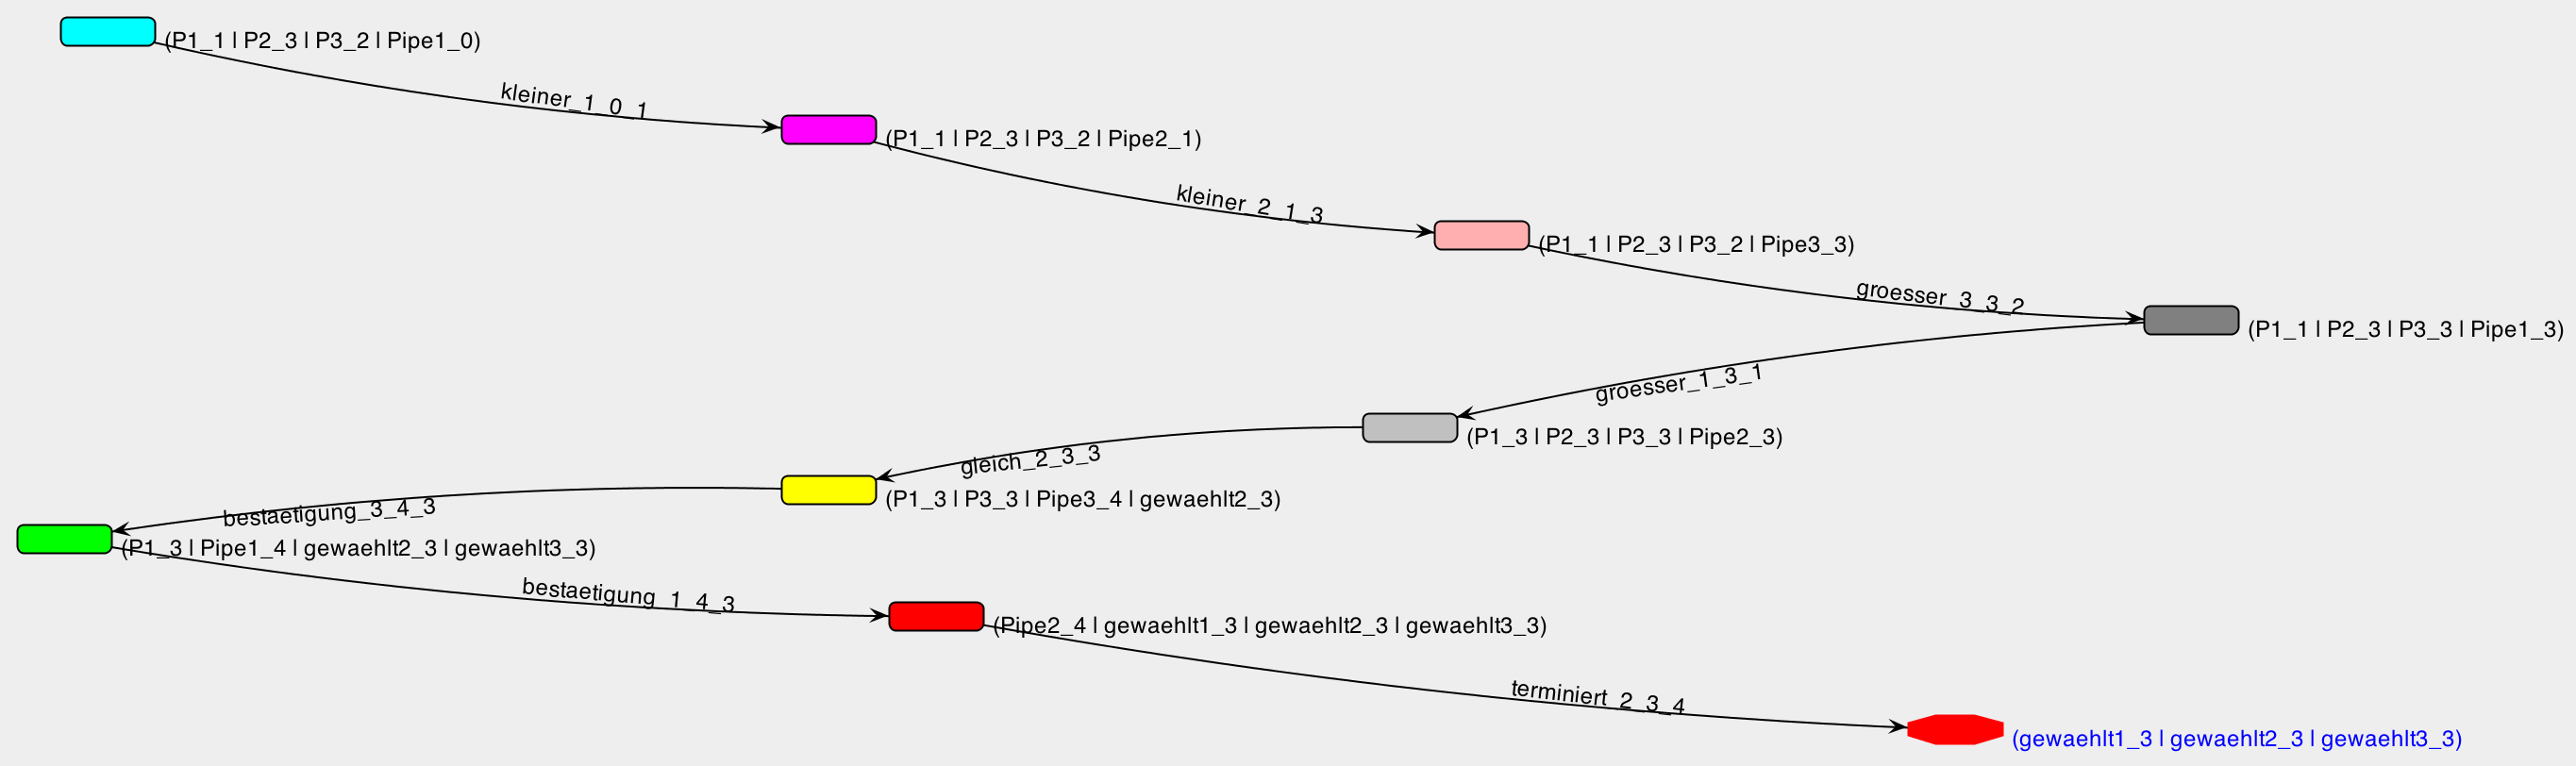
\includegraphics[width=1\linewidth]{img/reachibility_graph}
\caption{Erreichbarkeitsgraph des PN}
\label{fig:reachibility_graph}
\end{figure}

In Abbildung \ref{fig:reachibility_graph} ist der generierte Erreichbarkeitsgraph zu sehen. Es fällt auf, dass der Graph keine Abzweigungen hat, sondern nur einen Pfad enthält. Das bedeutet, dass der Algorithmus bei gleichen Bedingungen sich deterministisch verhält.

Würde man die Bedingungen verändern, sodass bspw. ein anderer Client den Master-Ausfall bemerkt oder ein anderer Client im Netzwerk hat die höchste ID, dann würde sich die Reihenfolge der Kanten im Erreichbarkeitsgraph verändern und die Knoten würden andere Stellen beinhalten. Der resultierende Erreichbarkeitsgraph wäre allerdings nach wie vor geradlinig.

\subsubsection{Prüfung durch CTL}
%TODO: Tabellen-Ref für Modell-Eigenschaften eintragen
Auf Grundlage des einfachen PN kann nun die Korrektheit in Bezug auf die Modell-Eigenschaften aus Tabelle X festgestellt werden. Die Übersicht über alle verwendeten Ausdrücke ist in Tabelle \ref{table:correctness_proof} im Anhang zu finden.

%TODO: Richtigen Namen des Token-Ring-Algorithmus einfügen
Die CTL-Ausdrücke lassen sich fehlerfrei auf das einfache Petri-Netz anwenden. Daher entspricht das erstellt CPN dem Token-Ring-Algorithmus von Chang\&Pang.
